%% define the main template style for the document
\documentclass{article}
%% import the NIPS package for LaTeX style
\usepackage[final]{nips_2017}

%% import packages that have custom options
\usepackage[utf8]{inputenc}
\usepackage[T1]{fontenc}
\usepackage[pagebackref=true]{hyperref}
\usepackage[nolist,nohyperlinks]{acronym}
\usepackage[section]{placeins}

%% Import general packages
\usepackage{
  amsmath, amssymb, amsfonts, nicefrac,
  algorithmic, textcomp, listings, url,
  graphicx, subfig, microtype,
  booktabs, longtable
}

%% start the document, the Markdown parser takes over from this point
\begin{document}
\title{Review: A Neural Algorithm of Artistic Style}

%% TODO: notations section?
%% TODO: clarify notations for both content and styl representation (N_l etc.)

\author{
    James C. Kauten \\
    Department of Software Engineering \\
    Auburn University \\
    Auburn, AL 36832 \\
    \texttt{kautenja@auburn.edu} \\
    \And
    Behnam Rasoolian \\
    Department of Industrial Engineering \\
    Auburn University \\
    Auburn, AL 36832 \\
    \texttt{bzr0014@auburn.edu} \\
}

\maketitle

\section{Paper Summary}

In their arXiv preprint, \textit{A Neural Algorithm of Artistic Style},
\cite{2015arXiv150806576G} prove a level of separability between the
\textit{content} of an image and the \textit{style} that characterizes it.
Using a \ac{CNN} trained to classify images on the ImageNet benchmark, they
transfer the style of famous works of art onto the content of arbitrary
photographs. They define loss functions between the activation maps of
various layers in the network that measure either content or style loss.
Minimizing the joint loss between a noise image $\textbf{x}$ and both a
content image $\textbf{p}$ and style image $\textbf{a}$ transfers the global
features of $\textbf{p}$, with the local styles of $\textbf{a}$ onto the
noise image $\textbf{x}$. Put simply, their algorithm paints photographs using
arbitrary works of art as a palette for colors and textures.


\subsection{Content Representation}

This work relies heavily on the understanding of convolutional layers. As a
collection of image filters, each layer extracts unique features from its
input image. As such, \cite{2015arXiv150806576G} postulate that as the layer
depth increases, the network cares more about the content of the image. That
is to say, deeper layers have a more specific understanding of what composes
a given image. Whereas, the shallower layers primarily understand the image
as raw pixels. This leads to their definition of \textit{content
representation} as the activations from deep layers in the network.

To objectively measure the difference of content between two images,
\cite{2015arXiv150806576G} define a loss function $\mathcal{L}_{content}$.
Given a content image $\textbf{p}$, a noise image $\textbf{x}$, and an
arbitrary layer $l$, the activations at $l$ for $\textbf{p}$ and $\textbf{x}$
are defined as $P^l$ and $F^l$ respectively. The squared euclidean distance
then measures the $\mathcal{L}_{content}$ loss between $P^l$ and $F^l$. Eq.
\ref{eq:content-loss} shows this loss function with an additional factor of
$\frac{1}{2}$ to simplify the formulation of the analytical gradient in Eq.
\ref{eq:content-grad}.

% TODO: note the M_l and N_l variables in the above paragraph
\begin{equation}
\label{eq:content-loss}
\mathcal{L}_{content}(\mathbf{p}, \mathbf{x}, l) =
\frac{1}{2} \sum_{i=1}^{N_l}\sum_{j=1}^{M_l}{(F^l_{ij} - P^l_{ij})^2}
\end{equation}

\begin{equation}
\label{eq:content-grad}
\frac{\partial \mathcal{L}_{content}}{\partial F^l_{ij}} =
\begin{cases}
    (F^l - P^l)_{ij} & \iff F^l_{ij} > 0 \\
    0 & \iff F^l_{ij} < 0 \\
\end{cases}
\end{equation}

\subsubsection{Content Reconstruction}

By back propagating the error from the $\mathcal{L}_{content}$ loss, we can
minimize the difference between a content image $\textbf{p}$ and a noise image
$\textbf{x}$ based on a given layer $l$. \cite{2015arXiv150806576G} find that
the second convolutional layer of the fourth block (\textit{block4\_conv2}) of
VGG19 produces the most desirable results.
% Fuck this sentence
Naturally, this is assessment is subjective to the beholders tastes.

To better understand the raw effect of this loss metric, we reconstructed an
image by taking the content loss at five separate layers in VGG19. We use the
first convolutional layer from each of the five blocks to produce the five
content reconstructions depicted in Fig. \ref{fig:content-reconstruction}. We
can see that the first three layers (block1\_conv1, block2\_conv1,
block3\_conv1) reproduce the input image in nearly full detail. However, the
fourth and fifth layers (block4\_conv1, block5\_conv1) reconstruct the image
with looser form. Deeper layers tend to work better for style transfer because
this looser representation allows the content to blend more smoothly with
other images while still preserving the global features of the content.

\begin{figure}[htp]
\centering
\caption{Content Reconstruction of \textit{T\"{u}bingen, Germany}}
\label{fig:content-reconstruction}

    \begin{minipage}{0.3\linewidth}
    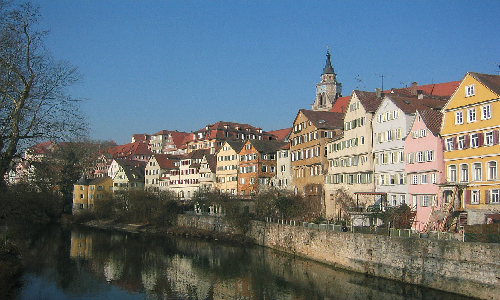
\includegraphics[width=\textwidth]{img/content/block1_conv1}
    \captionof*{figure}{block1 conv1}
    \end{minipage}
    \begin{minipage}{0.3\linewidth}
    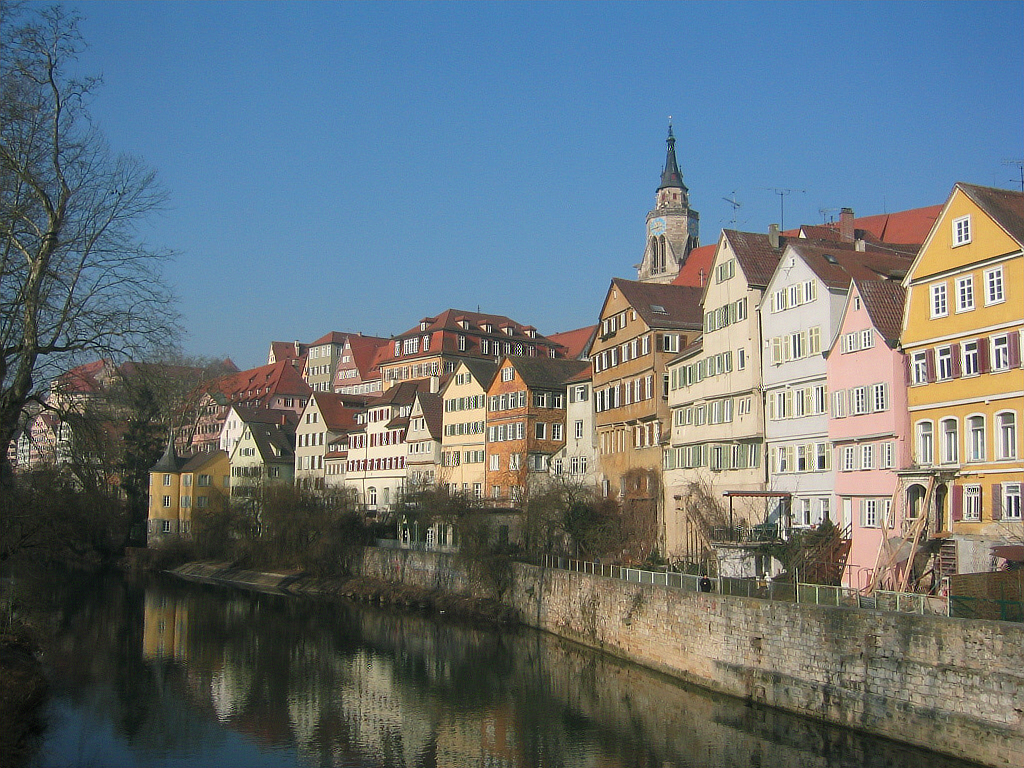
\includegraphics[width=\textwidth]{img/content/block2_conv1}
    \captionof*{figure}{block2 conv1}
    \end{minipage}
    \begin{minipage}{0.3\linewidth}
    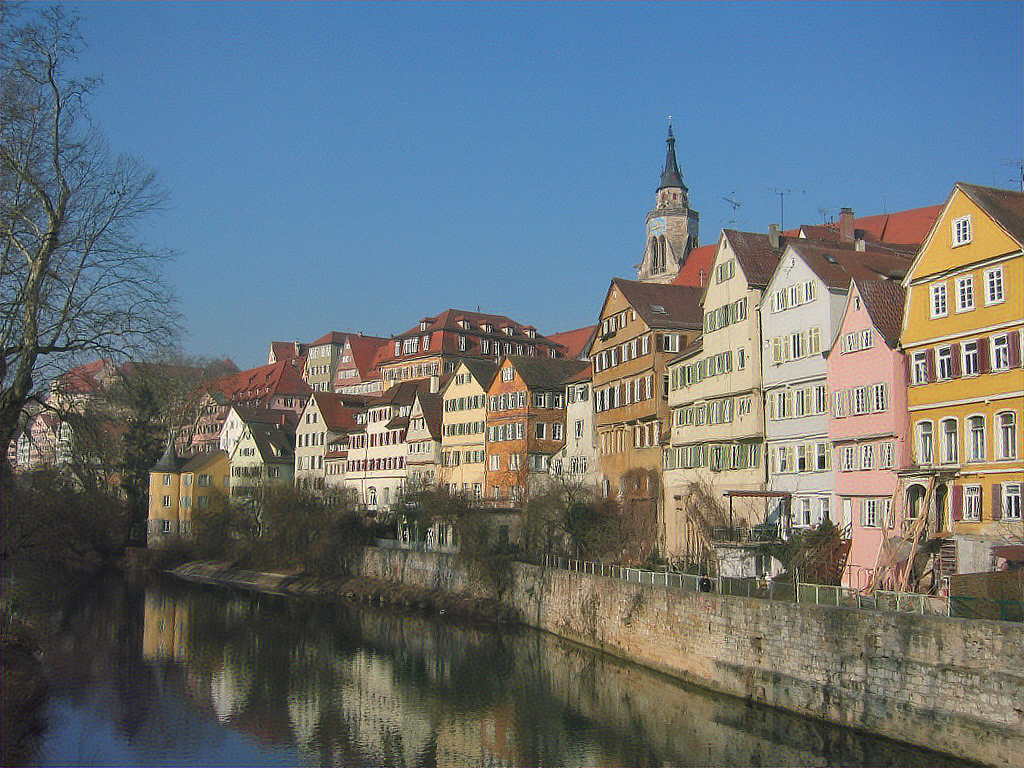
\includegraphics[width=\textwidth]{img/content/block3_conv1}
    \captionof*{figure}{block3 conv1}
    \end{minipage}

\medskip

    \begin{minipage}{0.3\linewidth}
    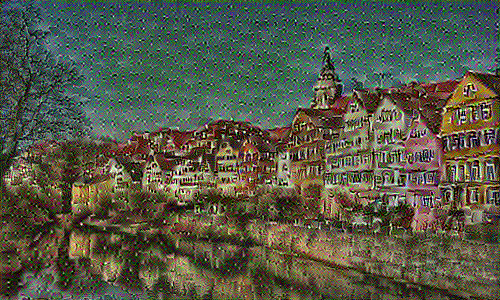
\includegraphics[width=\textwidth]{img/content/block4_conv1}
    \captionof*{figure}{block4 conv1}
    \end{minipage}
    \begin{minipage}{0.3\linewidth}
    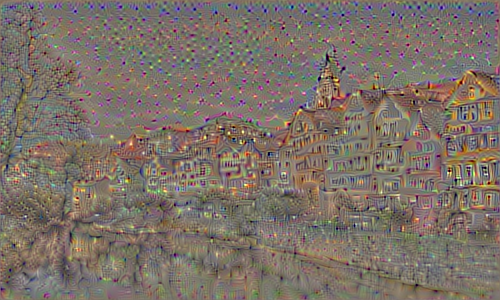
\includegraphics[width=\textwidth]{img/content/block5_conv1}
    \captionof*{figure}{block5 conv1}
    \end{minipage}

\end{figure}



\subsection{Style Representation}

Much like the content representation, style representation relies on the
feature responses of particular layers in the \ac{CNN}. However, this
representation uses a different feature space. Converting each activation
map to a \textit{gram matrix} allows the extraction of just the texture from
a given image. It does so by computing the correlations between different
filters in an arbitrary convolutional layer $l$. Simply put, the gram matrix
$G^l$ for an activation map is the inner product of feature maps:

\begin{equation}
G_{i j}^l = \sum_{k}^{M_l} F_{i k}^l F_{j k}^l
\end{equation}

With a new feature space representation of raw texture,
\cite{2015arXiv150806576G} define an additional loss function
$\mathcal{L}_{style}$ between an artwork image $\textbf{a}$, and a noise image
$\textbf{x}$ for some convolutional layer $l$. First, the activations at $l$
for $\textbf{a}$ and $\textbf{x}$ are transformed to their respective gram
matrices $A^l$, and $G^l$. Then, much like the content loss, we define
the style loss for a given layer as the squared euclidean distance between the
gram matrices $A^l$, and $G^l$:

\begin{equation}
E_l =
\frac{1}{4 N_l^2 M_l^2}
\sum_{i=1}^{N_l}\sum_{j=1}^{M_l}
(G^l_{ij} - A^l_{ij})^2
\end{equation}

\cite{2015arXiv150806576G} incorporate multiple layers in the style loss using
a weighted sum. In their experiments, they simply use a static weight
$w_l = \frac{1}{L}$ where $L$ is the number of layers contributing to the
style loss. Eq. \ref{eq:style-loss} displays the final formulation of the
$\mathcal{L}_{style}$ loss between $\textbf{a}$ and $\textbf{x}$ for some set
of layers bounded by $L$.

\begin{equation}
\label{eq:style-loss}
\mathcal{L}_{style}(\mathbf{a}, \mathbf{x}, L) = \sum_{l=0}^L w_l E_l
\end{equation}

Finally, we derive the gradient of this loss metric in Eq.
\ref{eq:style-grad}. Again, this gradient back propagates through the network
to provide a gradient of the loss with respect to the noise image
$\textbf{x}$.

\begin{equation}
\label{eq:style-grad}
\frac{\partial E_l}{\partial F^l_{ij}} =
\begin{cases}
    \frac{1}{N^2_l M^2_l}((F^l)^T (G^l - A^l))_{ji} & \iff F^l_{ij} > 0 \\
    0 & \iff F^l_{ij} < 0 \\
\end{cases}
\end{equation}

\subsubsection{Style Reconstruction}

\cite{2015arXiv150806576G} use the first convolutional layer of each block
(yielding five layers total) in their style loss. The selection of layers
for style reconstruction is similar to content reconstruction in that it is
subjective. To visualize the implications of layer selection, we reconstruct
style using five different sets of layers from VGG19. Fig.
\ref{fig:style-reconstruction} shows the output based on each of the five
sets. Unlike the content reconstruction, the style reconstruction preserves
none of the global content. Instead, it selects raw colors and textures from
the style, rearranging them around the new canvas $\textbf{x}$.

Like the content loss, additional layers provide a more in-depth understanding
of the style. The first convolutional layer of the first block seems to
extract simple points of color based on the color distribution of the style
$\textbf{a}$. As more layers contribute to the loss, the details of the
texture spread and smoothen across the noise image $\textbf{x}$.

\begin{figure}[htp]
\centering
\caption{Style Reconstruction of Vincent Van Gogh's \textit{A Starry Night}}
\label{fig:style-reconstruction}

    \begin{minipage}{0.3\linewidth}
    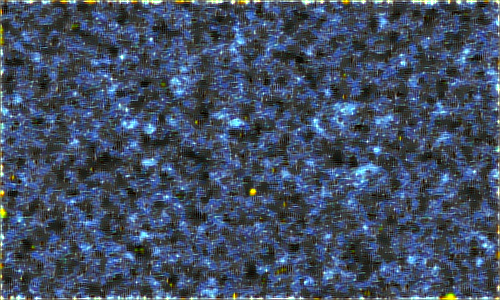
\includegraphics[width=\textwidth]{img/style/block1_conv1}
    \captionof*{figure}{block1 conv1}
    \end{minipage}
    \begin{minipage}{0.3\linewidth}
    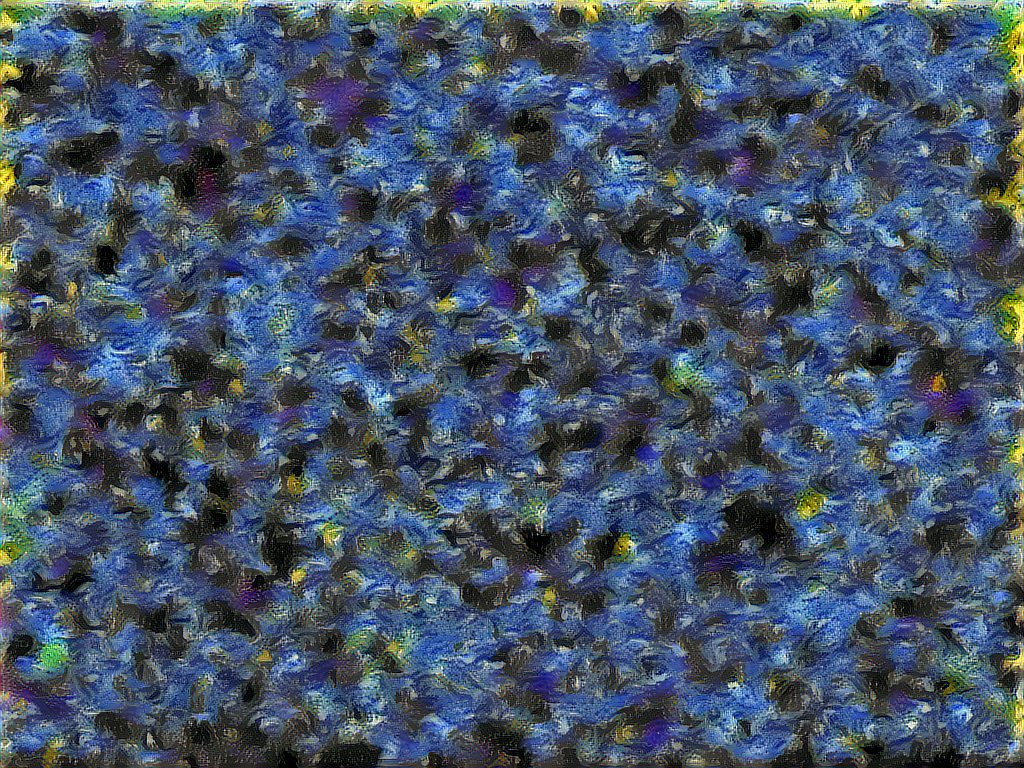
\includegraphics[width=\textwidth]{img/style/block2_conv1}
    \captionof*{figure}{block1,2 conv1}
    \end{minipage}
    \begin{minipage}{0.3\linewidth}
    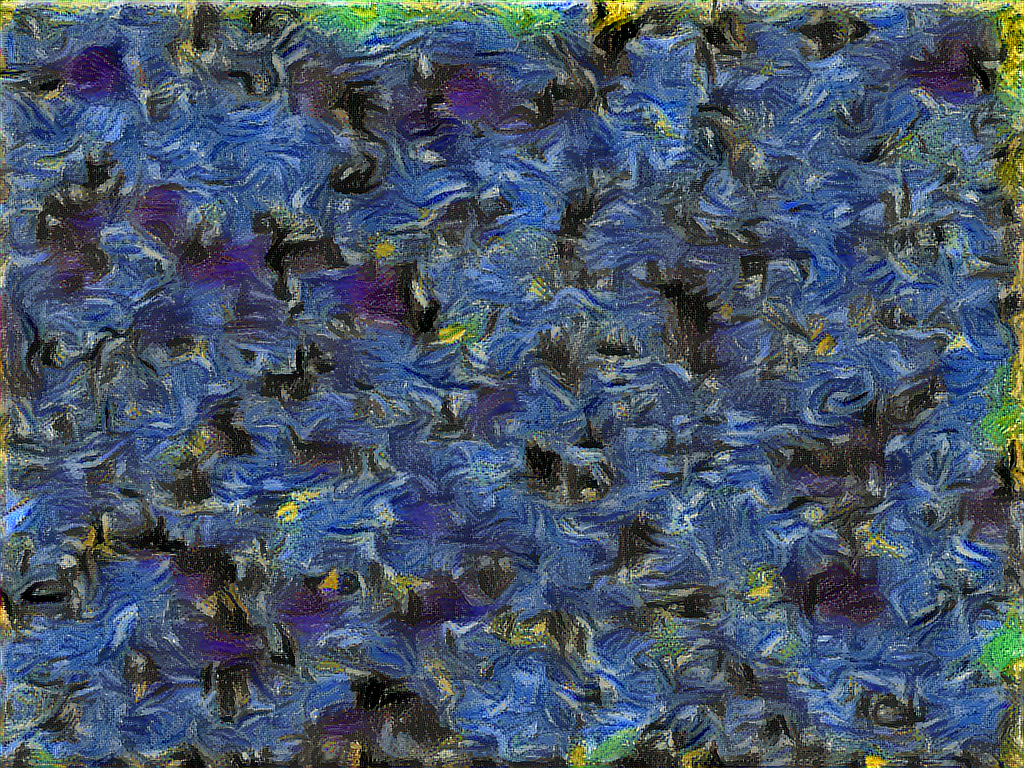
\includegraphics[width=\textwidth]{img/style/block3_conv1}
    \captionof*{figure}{block1,2,3 conv1}
    \end{minipage}

\medskip

    \begin{minipage}{0.3\linewidth}
    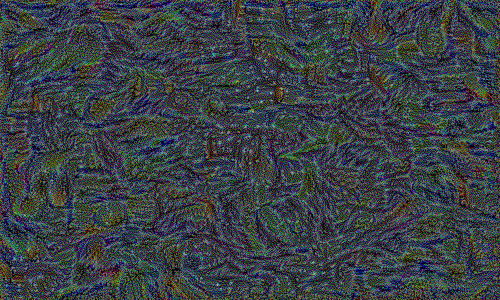
\includegraphics[width=\textwidth]{img/style/block4_conv1}
    \captionof*{figure}{block1,2,3,4 conv1}
    \end{minipage}
    \begin{minipage}{0.3\linewidth}
    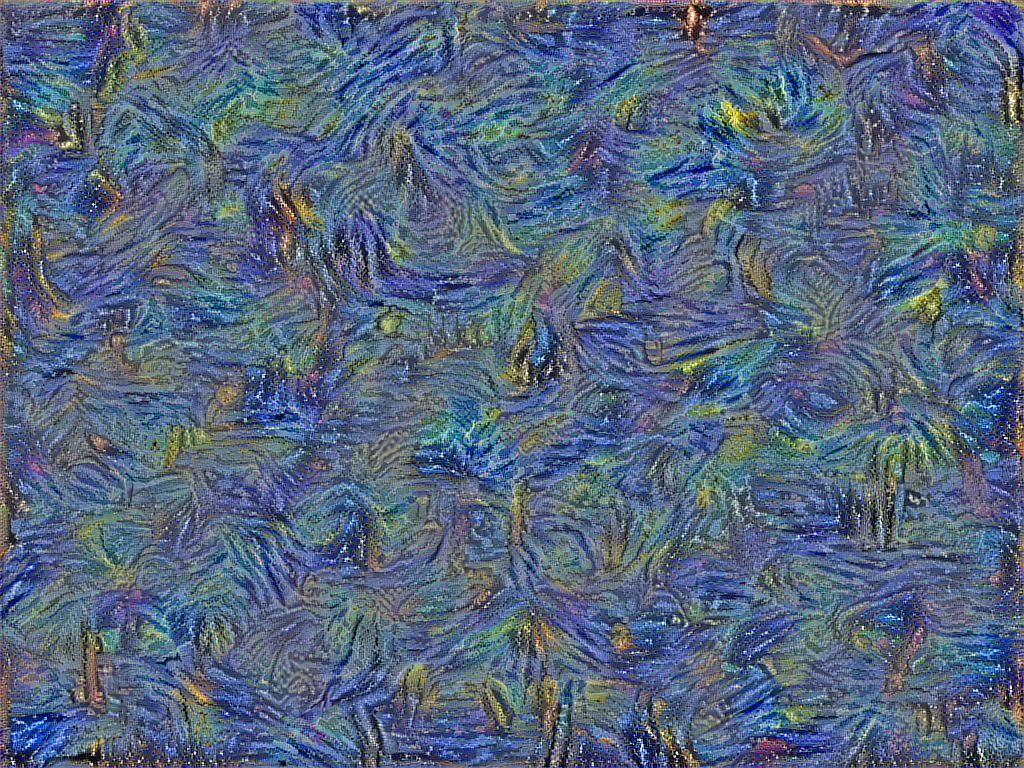
\includegraphics[width=\textwidth]{img/style/block5_conv1}
    \captionof*{figure}{block1,2,3,4,5 conv1}
    \end{minipage}

\end{figure}



\subsection{Transfer Representation}

With representations of style $\mathcal{L}_{style}$ and content
$\mathcal{L}_{content}$, we can form a final, blended, representation
$\mathcal{L}_{transfer}$ as the joint loss between the two. Eq.
\ref{eq:transfer-loss} shows a formulation of this loss metric using arbitrary
weighting factors $\alpha$ and $\beta$. \cite{2015arXiv150806576G} present no
technique for finding an optimal set of these parameters. However, they note
the best subjective results using a ratio $\frac{\alpha}{\beta} \in
[5e-4, 5e-3]$. All sets of $\alpha$ and $\beta$ with the same ratio will
produce the same results despite having differing values of
$\mathcal{L}_{transfer}$.

\begin{equation}
\label{eq:transfer-loss}
    \mathcal{L}_{transfer}(\mathbf{p}, \mathbf{a}, \mathbf{x}) =
    \alpha \mathcal{L}_{content}(\mathbf{p}, \mathbf{x}) +
    \beta \mathcal{L}_{style}(\mathbf{a}, \mathbf{x})
\end{equation}


\subsubsection{Style Transfer}

\cite{2015arXiv150806576G} use the same set of layers for each image they
present, but use differing values of $\alpha$ and $\beta$ to tune the results
to their liking. For content representation, they use block4 conv2. And, for
style representation, they use five layers with a weight of $\frac{1}{5}$
each: block1 conv1, block2 conv1, block3 conv1, block4 conv1, and block5
conv1. Oddly, our implementation produces vastly different results using the
same configuration and initial images. We believe this attributes to the
$\theta$ of VGG19 that we acquire from \cite{chollet2015keras} differing from
the $\theta$ of \cite{2015arXiv150806576G} that they likely came about
independently. Fig. \ref{fig:style-transfer} shows the results of the
algorithm for a single content image and four different styles.

\section{Strengths}

As the preliminary paper on neural style transfer, the strength of this work
lies in the novelty of the problem \& solution. \cite{2015arXiv150806576G}
loosely define a new problem of \textit{style transfer} and present an
optimization method for solving it. Although the \textit{transfer problem} had
been studied prior, no work had successfully blended styles with content in a
way that resembled a painting.

Despite involving complex technology, the actual method is beautifully simple.
Utilizing a network pre-trained to detect objects provides a strong analog to
a human artist. Different layer, hyperparameter, and initial noise selection,
resembles how different humans may experience similar things, but produce
vastly different artistic styles. This work may not focus on neuro-science,
but it provides a unique window into how visual creativity functions from a
purely mathematical perspective.



\section{Weaknesses}

Although the work of \cite{2015arXiv150806576G} shows many strengths, it
demonstrates a level of weakness as well. Because the problem they're solving
is loosely defined and largely based on subjective opinion, a truly objective
measure of either methods or solutions is unattainable. As such, comparing new
methods to this one presents a challenge for future work to dismantle.

Despite reporting the best results using L-BFGS to optimize noise,
\cite{2015arXiv150806576G} present no substantiation or comparative metrics
against other optimization techniques. It's understandable that they might
gloss over this detail given the subjectivity of the end result. But, it
seems to lack scientific rigor. We find that the Adam optimizer produces
better results at a fraction of the complexity, both computational, and
mathematical.

A final weakness of this solution is the complexity and wall clock time.
VGG19 is a large network with over 4M parameters making the optimization task
resource intensive. \cite{2015arXiv150806576G} note wall clock times of up to
an hour to produce single images running their algorithm on high-end GPUs.
However, using the Adam optimizer on a GTX1070, we were able to achieve good
results in $\approx 5$m. Additionally, high resolution images require
massive amounts of RAM. This ultimately results in bottlenecking as the GPU
falls back on system RAM if VRAM runs out. These limitations make it difficult
to process HD images or video in a reasonable amount of time.



\section{Future Work}

In a later publication, \cite{preserving-color-in-neural-style-transfer}
introduce two independent techniques for preserving the color from the content
during style transfer. The first method uses a simple linear transformation
before the algorithm starts to transfer the content's color to the style
image. The other technique utilizes the YIQ color space (opposed to the usual
RGB space) during the optimization to constrain style transfer to the
\textit{luminance} channel (Y). This essentially does the style transfer in
black and white, then fuses the IQ channels from the content image into the
stylized output image.

\cite{2016arXiv160308155J} improve upon the method in this paper by removing
the expensive optimization algorithm. Instead, they train a network to stylize
images in a single pass-through of the network. Using a TitanX GPU, their
network can style a content image in just $50ms$. This is a massive $7.2e4$x
faster than the reported time of \cite{2015arXiv150806576G} ($\approx 1h$).
This work  brings applications like real-time stylization closer to fruition.

\cite{kim2017learning} present a \ac{GAN} model for style transfer. The model
learns a mapping between two independent sets - their example uses
\textit{shoes} and \textit{handbags} - of images with no labeling information.
The trained model can then take a new image belonging to one set and produce
its complement in the other set. In other words, the model would input a
picture of a handbag, then output a picture of a new shoe bearing stylistic
similarities to the handbag.




\section{Questions \& Answers}

\paragraph{Layers Used in Loss Functions} \textit{Why do [the authors] use 5
convolutional layers? Could there be more or less?}

\cite{2015arXiv150806576G} select the 5 style layers based on their results
for style reconstruction. The five layers in question provide results that
they find the most aesthetically pleasing. That said, there can be as few as
1 layer used for style loss or as many as necessary. Fig.
\ref{fig:style-layers-effect} shows the effect of different sets of style
layers in the style loss. We see that the additional layers do in fact help
transfer more of the style.

\begin{figure}[htp]
\centering
\caption{Samford Hall Styled as Pablo Picasso's \textit{Seated Nude} Using
Different Style Loss Layer Sets}
\label{fig:style-layers-effect}

    \begin{minipage}{0.3\linewidth}
    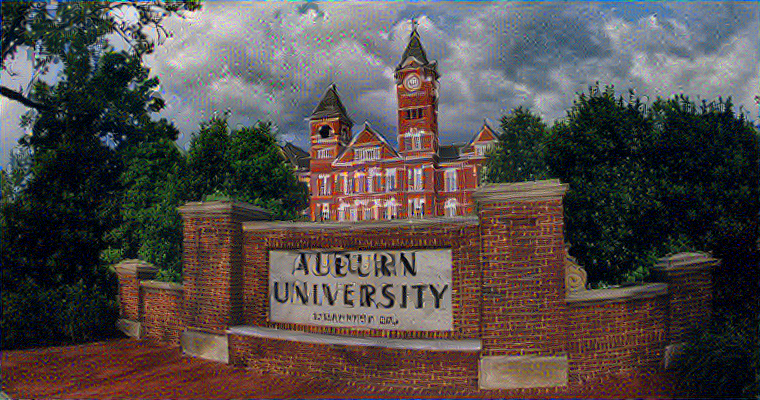
\includegraphics[width=\textwidth]{img/style-layer-selection/block1_conv1}
    \captionof*{figure}{block1 conv1}
    \end{minipage}
    \begin{minipage}{0.3\linewidth}
    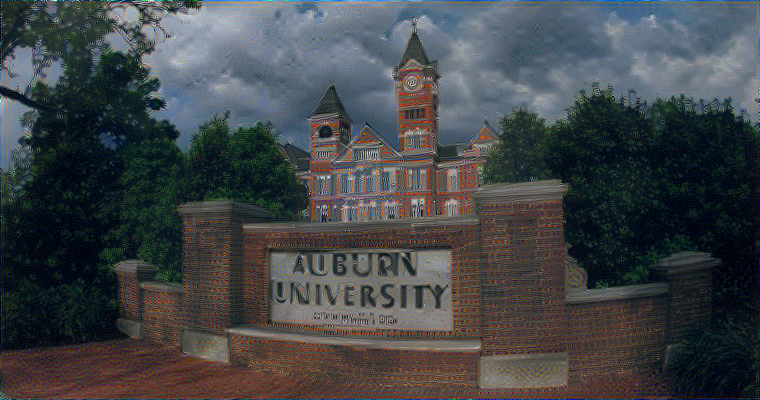
\includegraphics[width=\textwidth]{img/style-layer-selection/block2_conv1}
    \captionof*{figure}{block1,2 conv1}
    \end{minipage}
    \begin{minipage}{0.3\linewidth}
    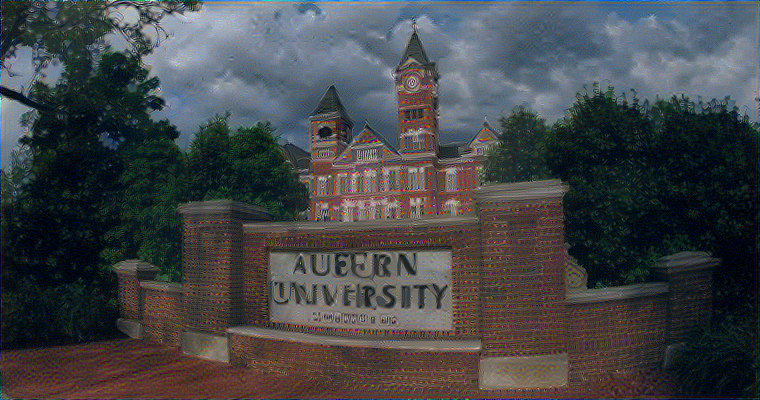
\includegraphics[width=\textwidth]{img/style-layer-selection/block3_conv1}
    \captionof*{figure}{block1,2,3 conv1}
    \end{minipage}

\medskip

    \begin{minipage}{0.3\linewidth}
    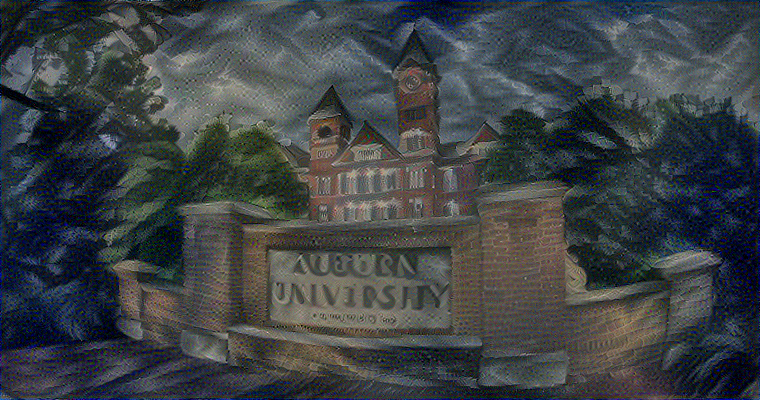
\includegraphics[width=\textwidth]{img/style-layer-selection/block4_conv1}
    \captionof*{figure}{block1,2,3,4 conv1}
    \end{minipage}
    \begin{minipage}{0.3\linewidth}
    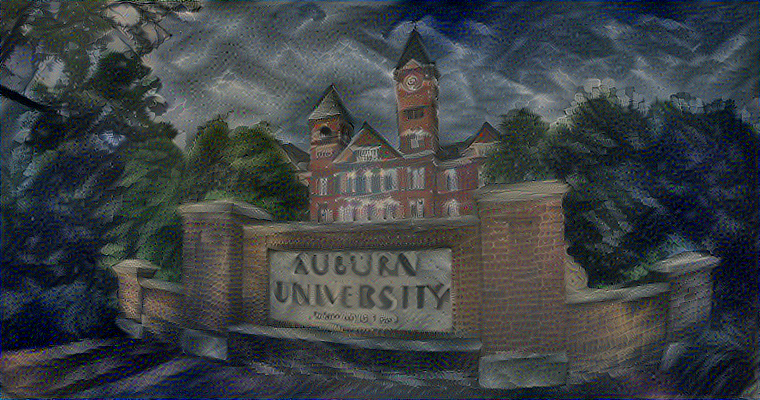
\includegraphics[width=\textwidth]{img/style-layer-selection/block5_conv1}
    \captionof*{figure}{block1,2,3,4,5 conv1}
    \end{minipage}

\end{figure}

For the content loss, they selection block4 conv2 because they find the
representation at this activation map allows the content to blend better with
the style. This provides a more realistic "painting" effect of the content by
smoothing out sharp lines and corners as if they were placed by a paint brush.
Fig. \ref{fig:content-layers-effect} shows the effect of using five different
layers for content loss. The first image portrays more of an overlaying effect
than a blending of styles. And, the last image contains almost no content,
instead blending it into the background. As such, the optimal layer must sit
somewhere between these. That said, "optimal" depends on the viewers' taste in
images.

\begin{figure}[htp]
\centering
\caption{Samford Hall Styled as Pablo Picasso's \textit{Seated Nude} Using
Different Content Loss Layers}
\label{fig:content-layers-effect}

    \begin{minipage}{0.3\linewidth}
    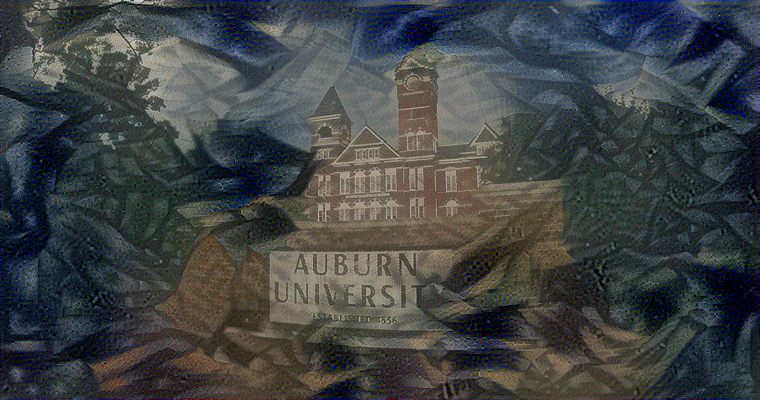
\includegraphics[width=\textwidth]{img/content-layer-selection/block1_conv1}
    \captionof*{figure}{block1 conv1}
    \end{minipage}
    \begin{minipage}{0.3\linewidth}
    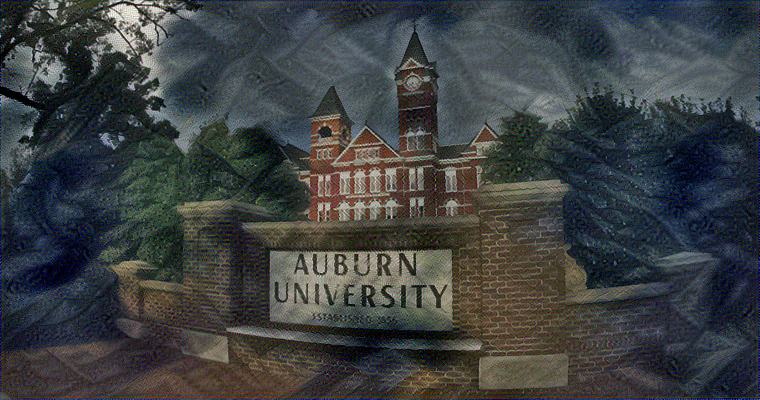
\includegraphics[width=\textwidth]{img/content-layer-selection/block2_conv1}
    \captionof*{figure}{block2 conv1}
    \end{minipage}
    \begin{minipage}{0.3\linewidth}
    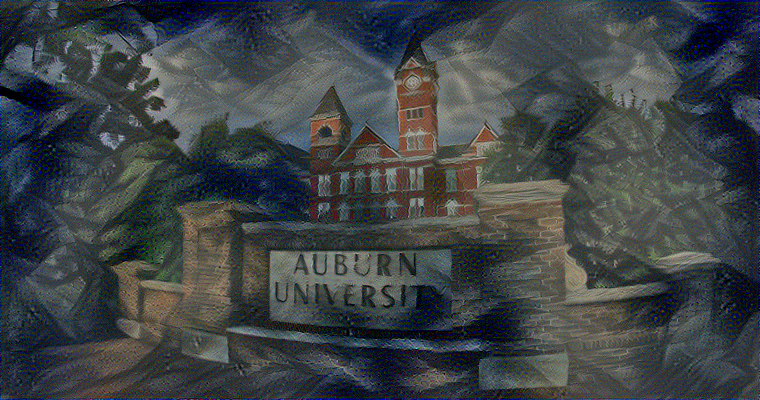
\includegraphics[width=\textwidth]{img/content-layer-selection/block3_conv1}
    \captionof*{figure}{block3 conv1}
    \end{minipage}

\medskip

    \begin{minipage}{0.3\linewidth}
    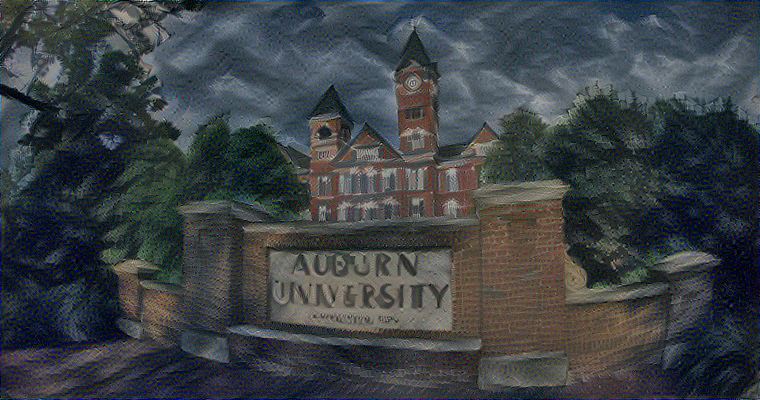
\includegraphics[width=\textwidth]{img/content-layer-selection/block4_conv1}
    \captionof*{figure}{block4 conv1}
    \end{minipage}
    \begin{minipage}{0.3\linewidth}
    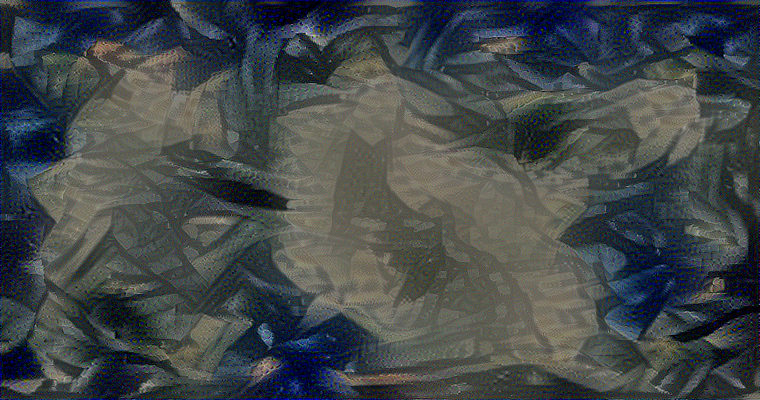
\includegraphics[width=\textwidth]{img/content-layer-selection/block5_conv1}
    \captionof*{figure}{block5 conv1}
    \end{minipage}

\end{figure}


\paragraph{Photo-realistic Style Transfer} \textit{Has there been any work to
use a real image as a style and transfer content to another content?}

\cite{gatys2016image} include a section on \textit{photo-realistic style
transfer} in the published version of \textit{A Neural Algorithm of Artistic
Style}. They find that they can transfer styles between content images with
relative success. As an example, Fig. \ref{fig:photo-realistic-style-transfer}
portrays how the algorithm can use a photo of New York at night to style a
photo of Atlanta at day, resulting in a new image of Atlanta at dusk.

\begin{figure}[htp]
\centering
\caption{Photo-realistic Style Transfer}
\label{fig:photo-realistic-style-transfer}
    \begin{minipage}{0.3\linewidth}
    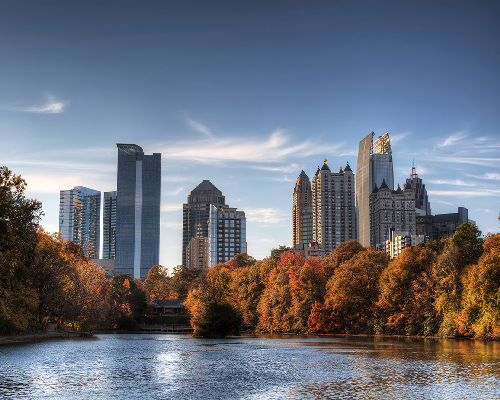
\includegraphics[width=\textwidth]{img/photo-transfer/p}
    \captionof*{figure}{$\textbf{p:}$ Atlanta at Day}
    \end{minipage}
    \begin{minipage}{0.3\linewidth}
    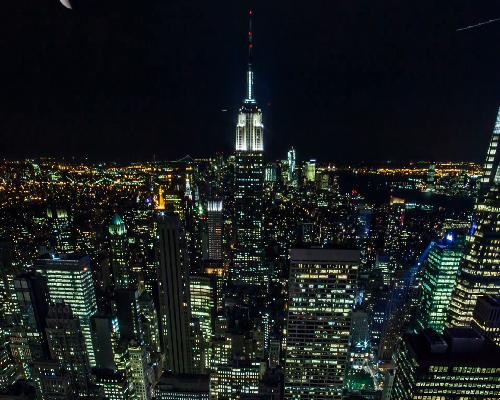
\includegraphics[width=\textwidth]{img/photo-transfer/a}
    \captionof*{figure}{$\textbf{a:}$ New York at Night}
    \end{minipage}
    \begin{minipage}{0.3\linewidth}
    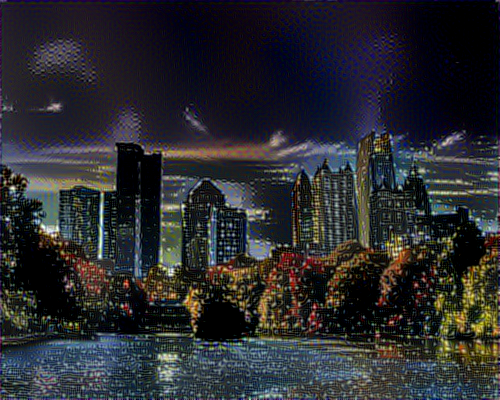
\includegraphics[width=\textwidth]{img/photo-transfer/x}
    \captionof*{figure}{$\textbf{x:}$ Atlanta at Dusk}
    \end{minipage}
\end{figure}


\paragraph{Affect of Transfer Learning} \textit{How does the choice of the
dataset affect the results?}

The model and dataset selection have a serious impact on the output results.
For instance, Fig. \ref{fig:alex-net-transfer} shows the effects of a GitHub
project by \cite{alexnet-transfer} using AlexNet. Contrary to the results
from VGG19, the AlexNet results hardly resembles either image, let alone a
transfer of style from one to another.

\begin{figure}[htp]
\centering
\caption{Style Transfer Using AlexNet}
\label{fig:alex-net-transfer}
    \begin{minipage}{0.3\linewidth}
    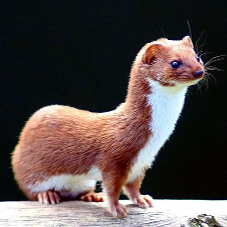
\includegraphics[width=\textwidth]{img/other-models/alex-net-p}
    \captionof*{figure}{$\textbf{p}$}
    \end{minipage}
    \begin{minipage}{0.3\linewidth}
    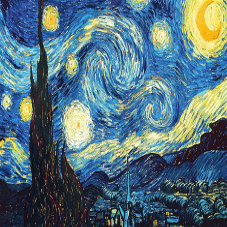
\includegraphics[width=\textwidth]{img/other-models/alex-net-a}
    \captionof*{figure}{$\textbf{a}$}
    \end{minipage}
    \begin{minipage}{0.3\linewidth}
    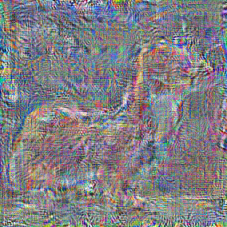
\includegraphics[width=\textwidth]{img/other-models/alex-net-x}
    \captionof*{figure}{$\textbf{x}$}
    \end{minipage}
\end{figure}

However, the \textit{Deep Dream} project of \cite{deep-dream} implements this
method on top of their \textit{Inception} architecture to great effect. Fig.
\ref{fig:deep-dream} shows Vincent Van Gogh's \textit{The Starry Night}
styled in a "deep dream".

\begin{figure}[htp]
\centering
\caption{\textit{Deep Dream}: Style Transfer Using Inception Net}
\label{fig:deep-dream}
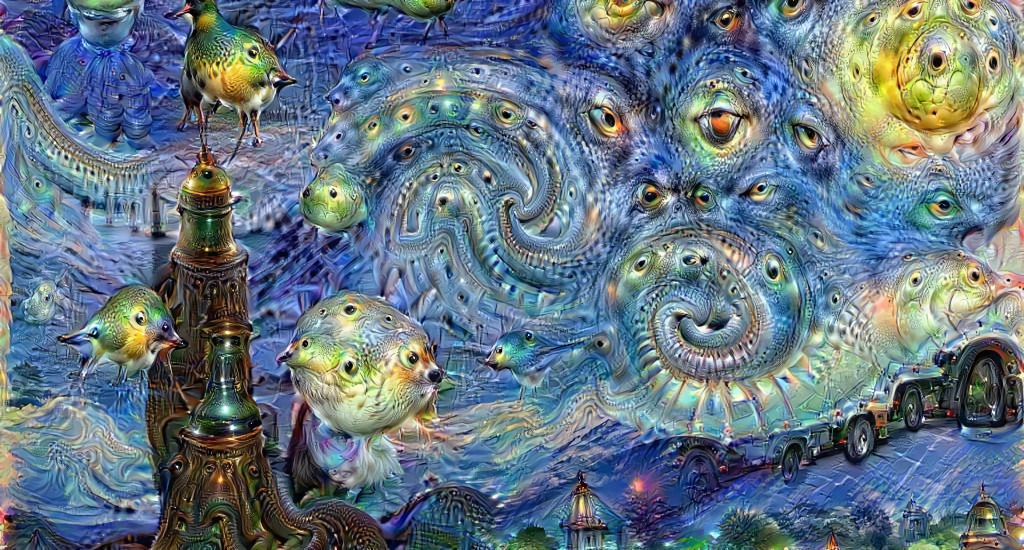
\includegraphics[width=0.9\textwidth]{img/deep-dream}
\end{figure}

\paragraph{Automatic Hyperparameter Selection} \textit{Has there been any
work to find an optimal configuration of layers automatically?}

Unfortunately, this work features abundant hyperparameters that must be tuned
manually on a per image basis. \cite{2017arXiv170108893R} respond to this
limitation with an automatic hyperparameter optimizer that dynamically
updates $\alpha$ and $\beta$ (and two other parameters unique to their joint
loss function) during the optimization process. However, their arXiv print
doesn't go into enough detail as to how to process functions.

\paragraph{Marketing and Social Media} \textit{Have their been any marketing
or social media campaigns utilizing this technology?}

\cite{2017arXiv170104928J} integrate impressionism into film using neural
style transfer. Interestingly, Kristen Stewart is a co-author for this paper.
Style transfer also appears in music videos by artists such as \cite{MGMT}.
Aside from these artistic applications, it doesn't seem that neural style
transfer has made an impact on advertising, marketing, and social media yet.

\paragraph{Dreamscope} \textit{Does Dreamscope (a mobile app) use this
neural method in their image filters?}

Their app store listing ambiguously states that they use cutting edge AI
techniques. However, articles confirm that at least one of their filters
utilizes Deep Dream, first presented by \cite{deep-dream}. Deep Dream, based
on the "Inception" network, uses the same transfer learning and optimization
technique to style images. However, the results are vastly different; Fig.
\ref{fig:deep-dream} shows how Deep Dream works by blending content (images,
buildings, etc.) into a style.

\paragraph{Camouflage} \textit{Are there any papers of this for hyper
localized camouflage?}

To the best of our finding, no current work focuses on the synthesis of new
camouflage patterns using this technique. However, \cite{camo-nn} present a
neural model for the detection of camouflage targets in an image. A potential
future research direction might explore using transfer learning in this domain
to produce new camouflage textures.

\paragraph{Style Transfer Detection} \textit{Is there any work on detecting
if this process has been applied to any image? i.e detecting the difference
between a real painting and a synthetic one?}

No current work attempts to detect whether a picture is genuine or synthetic.
An interesting future research direction might explore how to detect such a
phenomenon. One could potentially us a \ac{GAN} with a dataset of real and
synthetic artwork to learn the general differences between the real and fake
images.

\paragraph{Content as a Video} \textit{When this technique is applied to
videos, how do we ensure adjacent frames are similar enough to make the video
smooth?}

\cite{2016arXiv160408610R} study the potential of this method for styling
videos. They utilize \textit{optical flow} to ensure the motion perceived by
the sequence of frames is preserved. They initialize the first frame of the
video using random noise, but then recursively use the output from the last
frame as input for the next frame optimization. Additionally, they weight the
input frames by the joint combination of forward and backward optical flow to
focus the agitation of the noise to the moving regions between the frames.

\paragraph{Resource Consumption During Video Style Transfer} \textit{Knowing
that the current machine is slow to process a single frame, how can we
efficiently process video at $60fps$?}

The optimization technique discussed in these works is resource intensive
and slow. \cite{2016arXiv160308155J} combat this weakness by defining a faster
method. Opposed to optimizing a noise image using a network trained on
classification, they postulate training a network to do one-shot style
transfer of a noise image. That is to say, their network takes a content image
as input and outputs a stylized version in a single pass-through. Using an
nVidia TitanX, they are able to reduce the time to style a content image to
$\approx 50ms$ with no loss in transfer quality. Although this technique
looses the ability to quickly generalize to new styles, a production
application using a preset style could utilize this network to style videos at
$60fps$ in a reasonable amount of time. A future research direction might
explore reducing this time even further. A consistent $16ms$ per frame would
allow for real-time processing of frames at $\approx 60Hz$.


% MARK: bibliography
%% print the bibliography using the custom NIPS bib style
\bibliographystyle{my-unsrtnat}
\bibliography{references}



% MARK: appendix
% \appendix

\begin{figure}[ht]
\centering
\caption{Style Transfer}
\label{fig:style-transfer}

    \begin{minipage}{0.45\linewidth}
    \centering
    \captionof*{figure}{Content Image \textbf{p}, \textit{T\"{u}bingen, Germany}}
    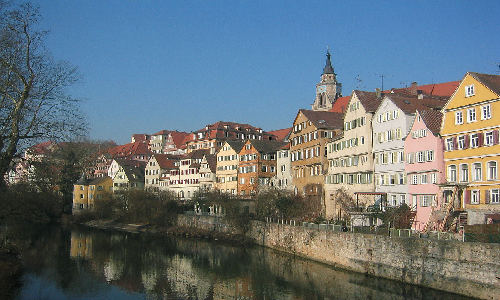
\includegraphics[width=0.9\textwidth,height=1.5in]{img/content/tubingen}
    \end{minipage}

\medskip

    \begin{minipage}{0.45\linewidth}
    \centering
    \captionof*{figure}{\textit{The Shipwreck of The Minotaur}}
    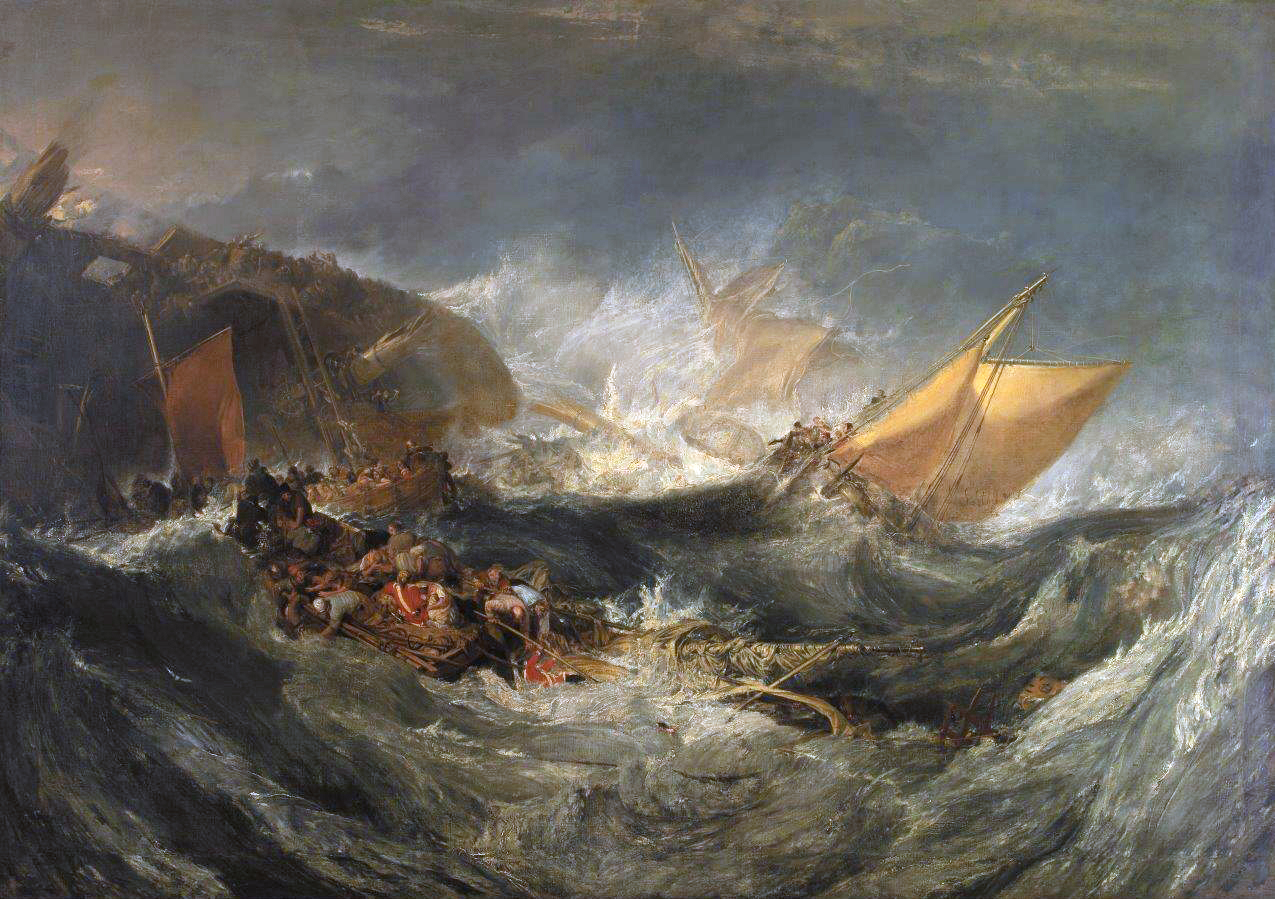
\includegraphics[width=0.9\textwidth,height=1.5in]{img/artworks/the-shipwreck-of-the-minotaur}
    \end{minipage}
    \begin{minipage}{0.45\linewidth}
    \centering
    \captionof*{figure}{Transfer Image \textbf{x}}
    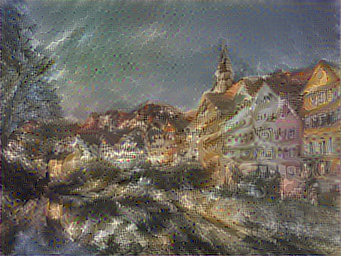
\includegraphics[width=0.9\textwidth,height=1.5in]{img/transfer/the-shipwreck-of-the-minotaur}
    \end{minipage}

\medskip

    \begin{minipage}{0.45\linewidth}
    \centering
    \captionof*{figure}{\textit{The Starry Night}}
    \includegraphics[width=0.9\textwidth,height=1.5in]{img/artworks/the-starry-night}
    \end{minipage}
    \begin{minipage}{0.45\linewidth}
    \centering
    \captionof*{figure}{Transfer Image \textbf{x}}
    \includegraphics[width=0.9\textwidth,height=1.5in]{img/transfer/the-starry-night}
    \end{minipage}

\medskip

    \begin{minipage}{0.45\linewidth}
    \centering
    \captionof*{figure}{\textit{Seated Nude}}
    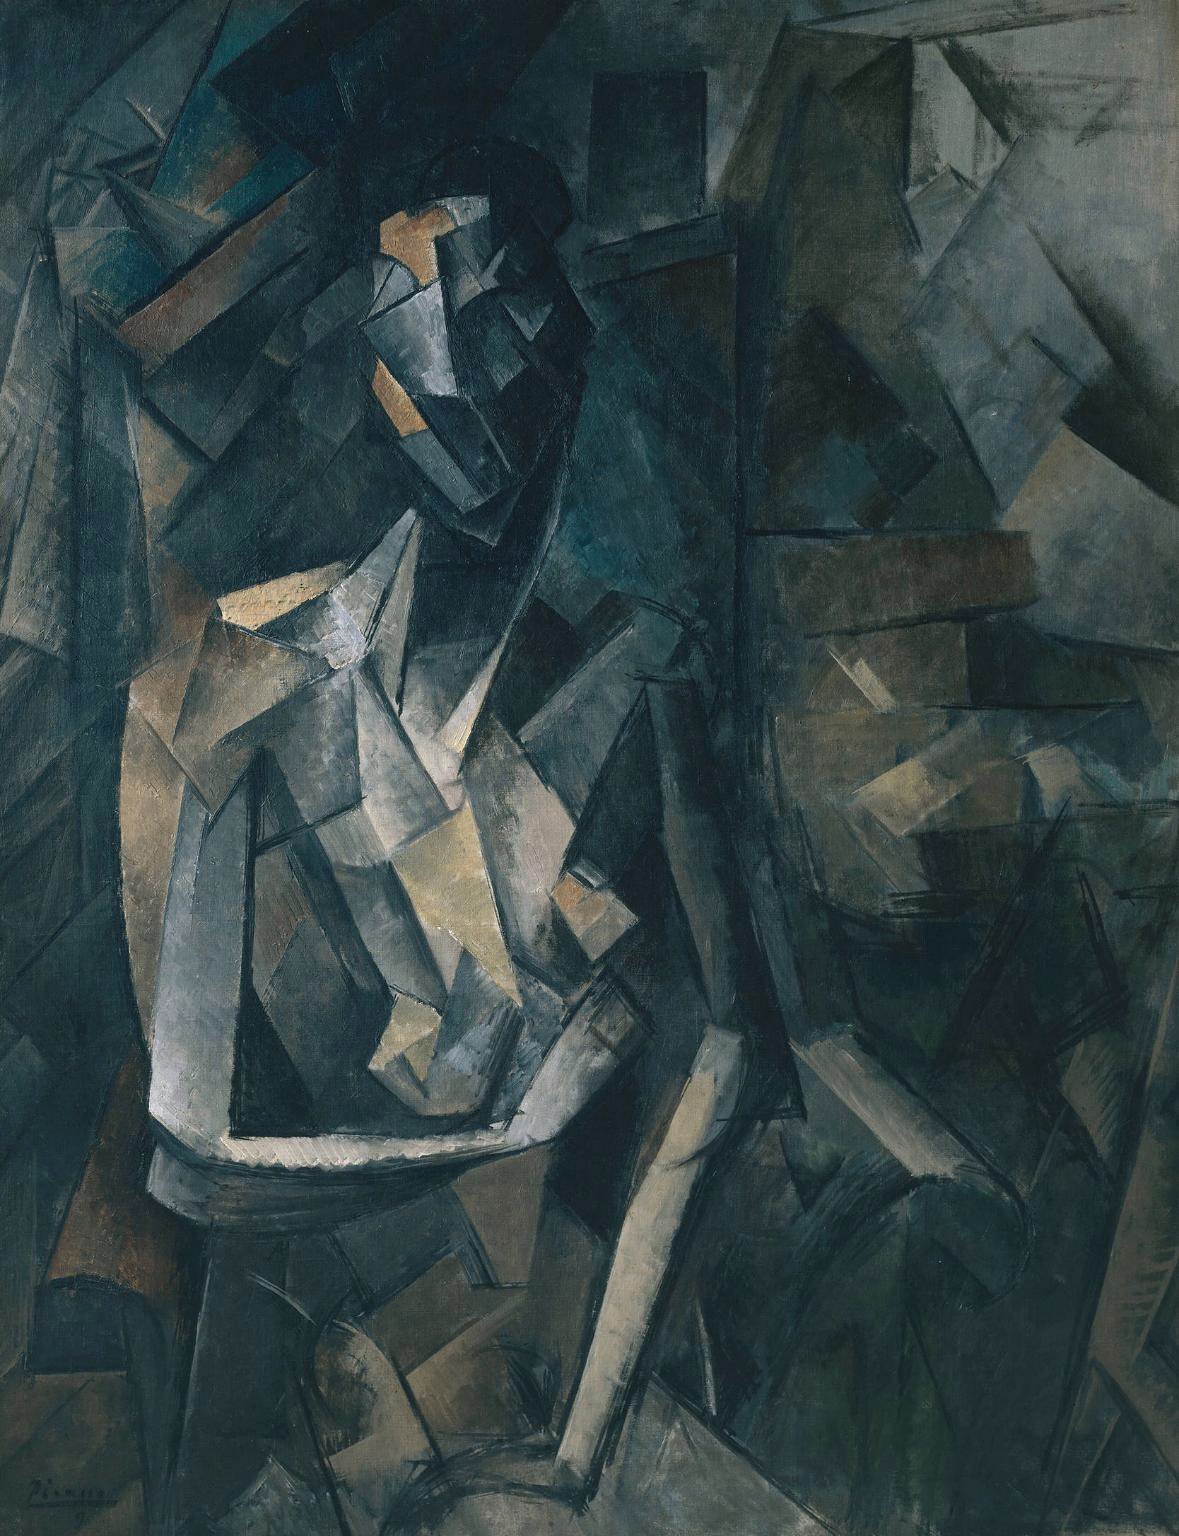
\includegraphics[width=0.9\textwidth,height=1.5in]{img/artworks/seated-nude}
    \end{minipage}
    \begin{minipage}{0.45\linewidth}
    \centering
    \captionof*{figure}{Transfer Image \textbf{x}}
    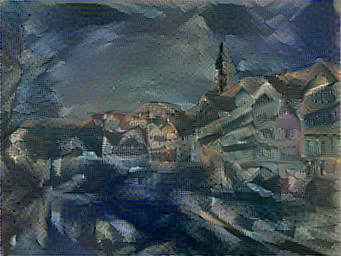
\includegraphics[width=0.9\textwidth,height=1.5in]{img/transfer/seated-nude}
    \end{minipage}

\medskip

    \begin{minipage}{0.45\linewidth}
    \centering
    \captionof*{figure}{\textit{The Scream}}
    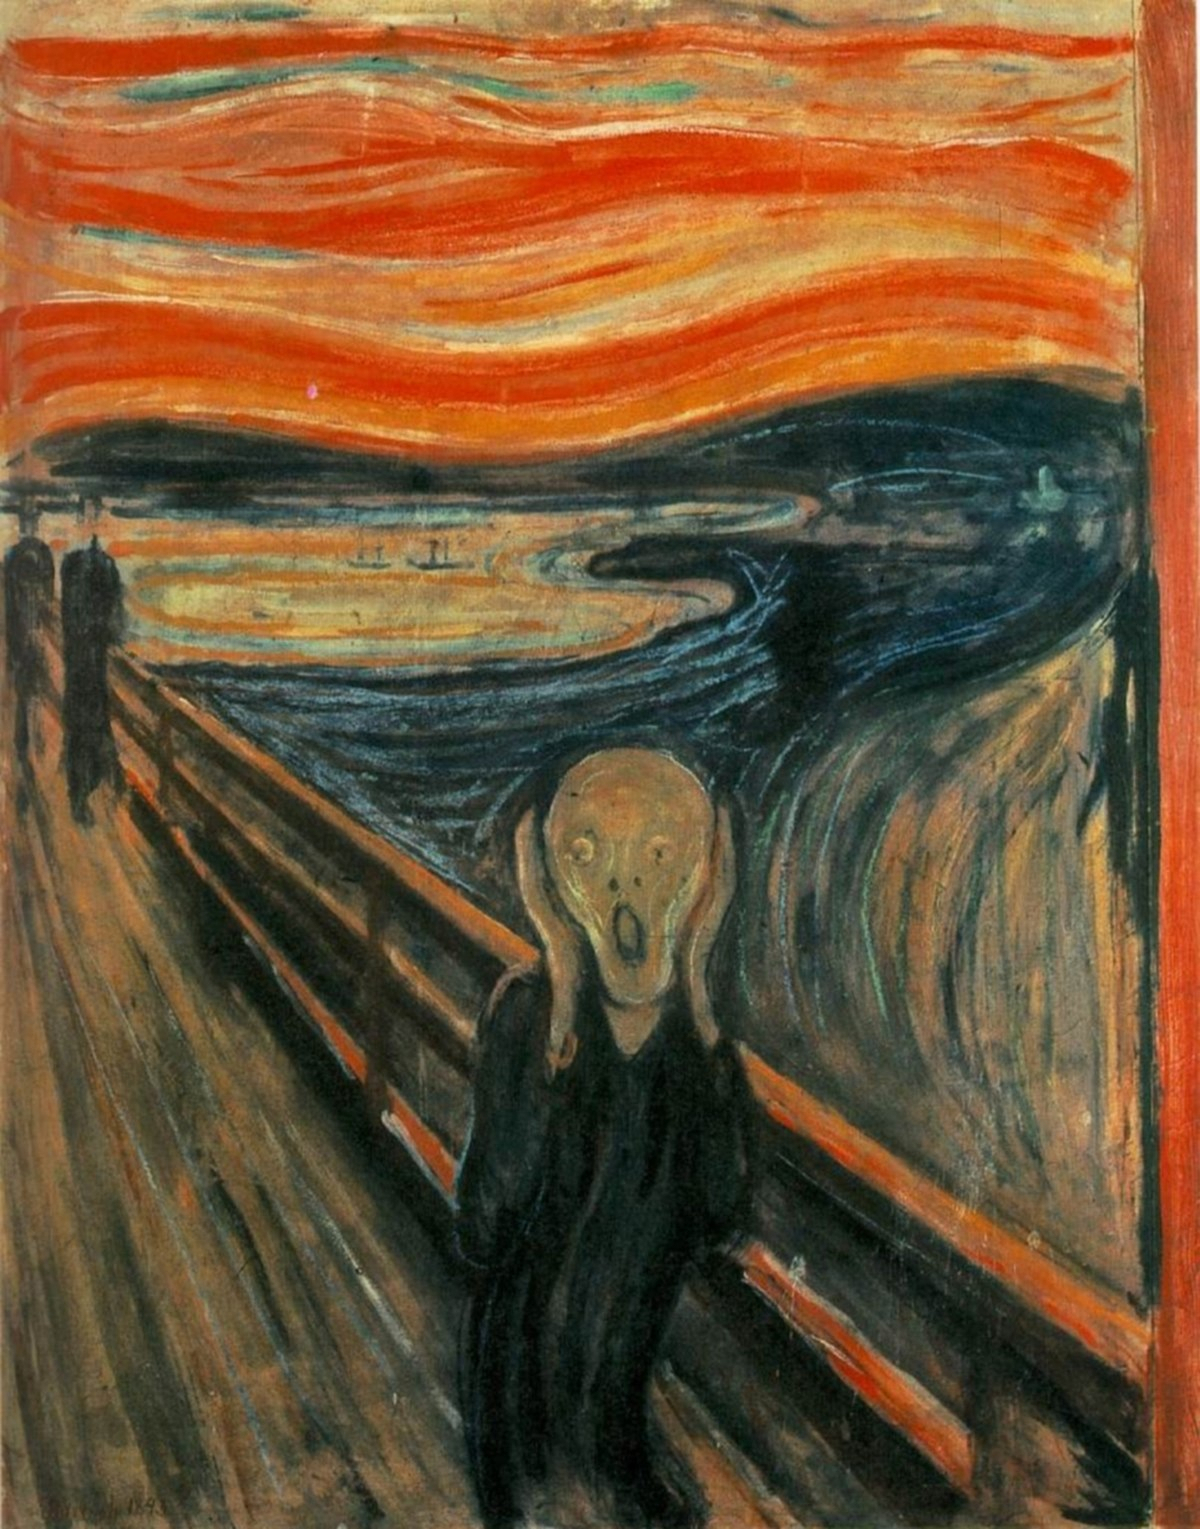
\includegraphics[width=0.9\textwidth,height=1.5in]{img/artworks/the-scream}
    \end{minipage}
    \begin{minipage}{0.45\linewidth}
    \centering
    \captionof*{figure}{Transfer Image \textbf{x}}
    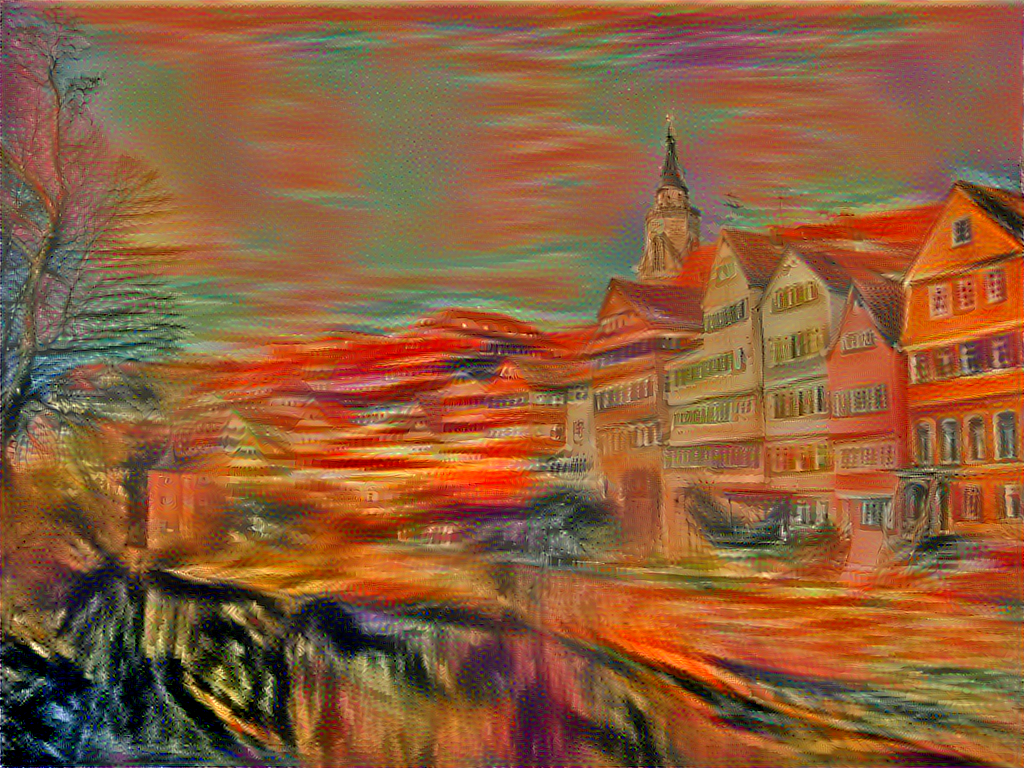
\includegraphics[width=0.9\textwidth,height=1.5in]{img/transfer/the-scream}
    \end{minipage}

\end{figure}



% MARK: acronyms
% a collection of Acronyms
\begin{acronym}
\acro{CNN}{Convolutional Neural Network}
\acro{GAN}{Generative Adversarial Network}
\end{acronym}

\end{document}
